\documentclass{article}
\usepackage{amsmath}
\usepackage{amssymb}
\usepackage{graphicx}
\usepackage{hyperref}
\usepackage[version=4]{mhchem}


\begin{document}
\section*{Problem}
In a convex quadrilateral \(A B C D, A D / / B C\). Show that \(A C \perp B D\) if \(A C^{2}+B D^{2}=(A D+B C)^{2}\).\\
\centering
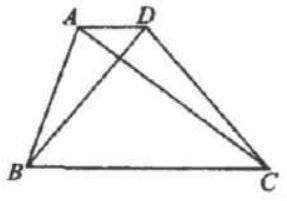
\includegraphics[width=\textwidth]{images/128(3).jpg}

\section*{Solution}
Draw \(D E\) so that \(D E / / A C\) and \(D E\) meets the extension of \(B C\) at \(E\). Then \(\triangle C E D \cong\) \(\triangle D A C\) and \(D E=A C, C E=A D\).

In \(\triangle B D E, B E=B C+C E=B C+A D . A D C E\) is a parallelogram and \(D E=A C\).

Since \(A C^{2}+B D^{2}=(A D+B C)^{2}\), or \(D E^{2}+B D^{2}=B E^{2}\),\\
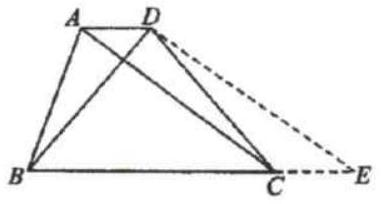
\includegraphics[width=\textwidth]{images/138(1).jpg} by the converse of the Pythagorean theorem, \(\angle B D E=90^{\circ}\).\\
Therefore \(B D \perp D E\). We also know that \(A C / / D E\), so \(A C \perp B D\).

\end{document}
